\documentclass[11pt,a4paper]{article}

\usepackage{../../templates/style}

\begin{document}

\begin{problem}{Temperature is Rising}{standard input}{standard output}{1 second}{1 megabytes}

เทือกเขาคุโรมาตี้มีพื้นที่เป็นรูปสี่เหลี่ยมจัตุรัสขนาด $M \times M$ ตารางเมตร และมีอุณหภูมิแตกต่างกันในแต่ละตารางเมตร นักเดินทางหญิงเริ่มเดินทางจากตำแหน่งหนึ่งในเทือกเขาแห่งนี้ โดยจากตำแหน่งใดๆ ก็ตาม เธอสามารถเลือกเดินทางไปในทิศเหนือ (N) ตะวันออก (E) ใต้ (S) และ ตะวันตก (W) ครั้งละ $1$ เมตร แต่ตำแหน่งที่เธอจะเดินไปนั้นจะต้องมีอุณหภูมิสูงกว่าตำแหน่งที่เธออยู่ในปัจจุบัน และไม่ใช่เขตหวงห้าม

ข้อมูลนำเข้าประกอบด้วยขนาดของเทือกเขา $M$ พิกัดเริ่มต้น $X$ และ $Y$ ซึ่งไม่ใช่เขตหวงห้าม และอุณหภูมิ $T$ $(–5 \leq T \leq 37)$ ในแต่ละตารางเมตรของเทือกเขาแห่งนี้ มีหน่วยเป็นองศาเซลเซียส (°C) โดยถ้าเป็นเขตหวงห้ามพิกัดนั้นจะถูกแทนด้วยตัวเลข $100$
\bigskip

\textbf{ตัวอย่าง} เทือกเขาขนาด $4 \times 4$ ตารางเมตร แสดงเส้นทางทั้งหมดของหญิงนักเดินทาง


\begin{figure}[h]
\centering
\begin{subfigure}{40ex}
\centering
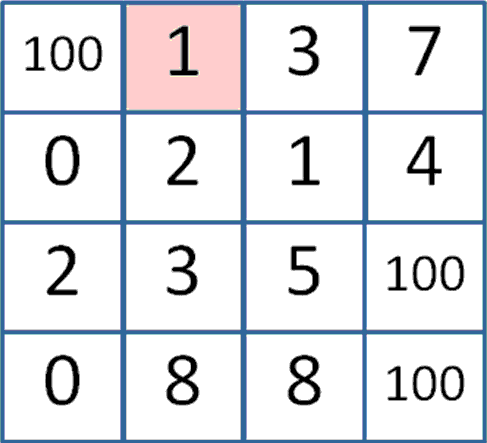
\includegraphics[width=25ex]{../latex/img/1061/1061-1.png}
\caption*{กำหนดให้จุดเริ่มต้นที่ $X = 2$ และ $Y = 1$}
\end{subfigure}%
\begin{subfigure}{40ex}
\centering
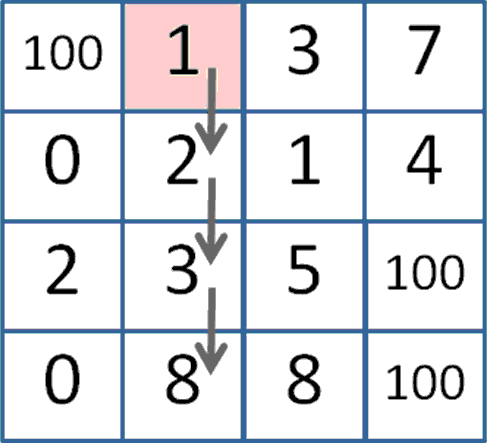
\includegraphics[width=25ex]{../latex/img/1061/1061-2.png}
\caption*{เส้นทางแรก อุณหภูมิสูงสุดเท่ากับ $8$ °C}
\end{subfigure}%

\end{figure}


\begin{figure}[h]
\centering
\begin{subfigure}{40ex}
\centering
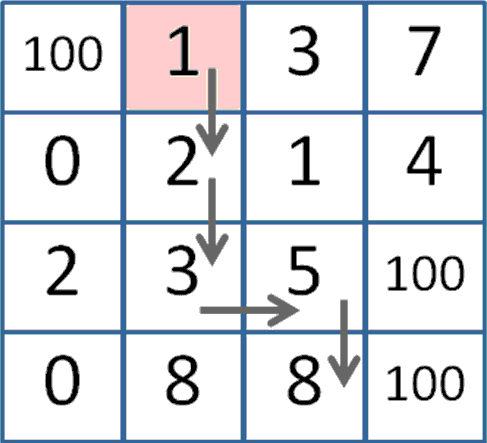
\includegraphics[width=25ex]{../latex/img/1061/1061-3.png}
\caption*{เส้นทางที่สอง อุณหภูมิสูงสุดเท่ากับ $8$ °C}
\end{subfigure}%
\begin{subfigure}{40ex}
\centering
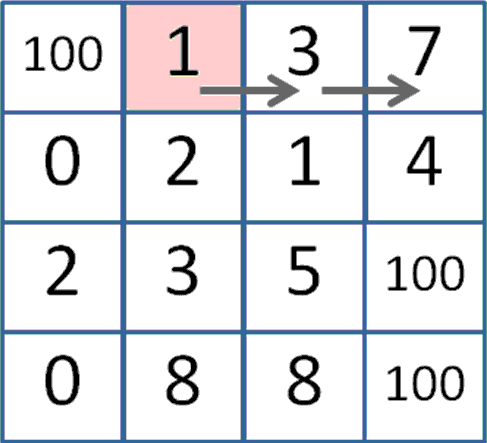
\includegraphics[width=25ex]{../latex/img/1061/1061-4.png}
\caption*{เส้นทางที่สาม อุณหภูมิสูงสุดเท่ากับ $7$ °C}
\end{subfigure}%
\end{figure}

จากตัวอย่างจะเห็นว่าในบรรดาเส้นทางทั้งหมด จุดที่มีอุณหภูมิสูงสุดที่นักเดินทางไปถึงก็คือ $8$ °C

\bigskip
\underline{\textbf{โจทย์}}  จงเขียนโปรแกรมหาอุณหภูมิสูงสุดที่เป็นไปได้ ที่เธอสามารถเดินทางไปถึง

\InputFile

\textbf{บรรทัดแรก} ขนาดความกว้าง (ยาว) ของเทือกเขา $M$ $(1 \leq M \leq 20)$

\textbf{บรรทัดที่สอง} รับข้อมูลพิกัดเริ่มต้น $(X, Y)$ $(1 \leq X \leq M;1 \leq Y \leq M)$ คั่นด้วยช่องว่าง โดยมุมซ้ายบนคือพิกัด $(1, 1)$

\textbf{บรรทัดที่ $3$ ถึง $M+2$} ในบรรทัดที่ $i+2$ ให้รับข้อมูลเทือกเขาในแถวที่ $i$ แต่ละบรรทัดมีตัวเลขจำนวนเต็ม $M$ จำนวน คั่นด้วยช่องว่าง แต่ละจำนวนแสดงอุณหภูมิ $T$ $(–5 \leq T \leq 37)$ หรือตัวเลข $100$ ถ้าเป็นเขตหวงห้าม


\OutputFile

\textbf{มีบรรทัดเดียว} แสดงอุณหภูมิสูงสุดที่เป็นไปได้ ที่นักเดินทางสามารถไปถึง

\Examples

\begin{example}
\exmp{4
2 1
100 1 3 8
0 2 1 4
2 3 5 100
0 8 8 100}{8}%
\exmp{1
1 1
9}{9}%
\exmp{5
4 2
0 1 100 100 0
100 2 3 1 1
100 100 4 5 100 
8 7 100 6 100
7 100 100 100 9}{6}%
\end{example}


\Source

การแข่งขันคอมพิวเตอร์โอลิมปิกสอวน.ครั้งที่ 4 ปี 2551 วันที่ 1

\end{problem}

\end{document}